\documentclass[twocolumn,dvipsnames]{article}

\usepackage{float}
% \usepackage[pdftex,dvipsnames]{xcolor}
\usepackage{tikz}
\usepackage{booktabs}
\usepackage{multirow}
\usepackage{lipsum,adjustbox}
\usepackage{array,url,lipsum}
\usepackage[utf8]{inputenc}
\usepackage[english]{babel}
\usepackage{multicol}
\usepackage{amsthm}
\usepackage{amsmath}
\usepackage{amssymb}
\usepackage{amsfonts}

\usepackage[colorinlistoftodos,prependcaption,textsize=tiny]{todonotes}

\usetikzlibrary{shapes.geometric} % required for the ellipse shape
\usetikzlibrary{calc,positioning}
\usetikzlibrary{fit, arrows, backgrounds, calc, hobby, positioning}

\newcommand\len[1]{\left|#1\right|}

\tikzset{vertex style/.style={%
    draw=#1,
    thin,
    fill=#1!70,
    text=white,
    minimum width=1cm,
    minimum height=1cm,
    outer sep=1pt,
    scale=0.5
  },
  text style/.style={%
    sloped,
    text=black,
    above
  }
}

\graphicspath{{img/}}
\DeclareGraphicsExtensions{.pdf,.jpeg,.png,.jpg}

\usepackage[
    backend=biber,
    style=numeric
]{biblatex}

\addbibresource[]{ML.bib}

\begin{document}
\twocolumn[{%
    \centering
        \LARGE Music By Genre: an Application Of Binary Classification Algorithms \\[1.5em]
        \large John Connor, Denis Khryashchev, Ari Mermelstein\\[1em]
        \normalsize
        \begin{tabular}{*{2}{>{\centering}p{.25\textwidth}}}
    \end{tabular}\\[3em]
}]

\begin{abstract}
In this paper we perform a binary classification of music by genre.
Music classification is an interesting and notoriously difficult problem.
In this paper we compare two methods of binary classification:
Soft Margin Support Vector Machines, and LASSO Regression.
We also explore feature selection,
including a novel chord normalization algorithm.
\end{abstract}

\section{Approach}
While there has been a great deal of significant research in the classification of music by genre,
most of the methods have required deep insights and a non-trivial amount of software development to extract the necessary features.
For example,~\cite{li2003comparative}, and the excellent textbook~\cite{weihs2016music}.

To this end, we have chosen the music21 python library~\cite{cuthbertMusic21} for the reading of midi files and the extraction of features.
The music21 API is easy to use and well documented, making it ideal for exploratory feature identification and extraction.
Unfortunately, the library is rather slow when it comes to the bulk manipulation of data.
(The slowness and idiosyncrasies of the music21 library were the main impediments to using additional features and classifying larger corpora.)
We use ScikitLearn~\cite{scikitLearn} to implement a support vector machine and to perform a LASSO regression,
and to automate the training and testing.
The MIDI files used were provided by Kunst der Fuge~\cite{wwwKunstderfuge} and MIDI DB~\cite{wwwMidiDb}.

\begin{figure}[h!]
    % \centering
      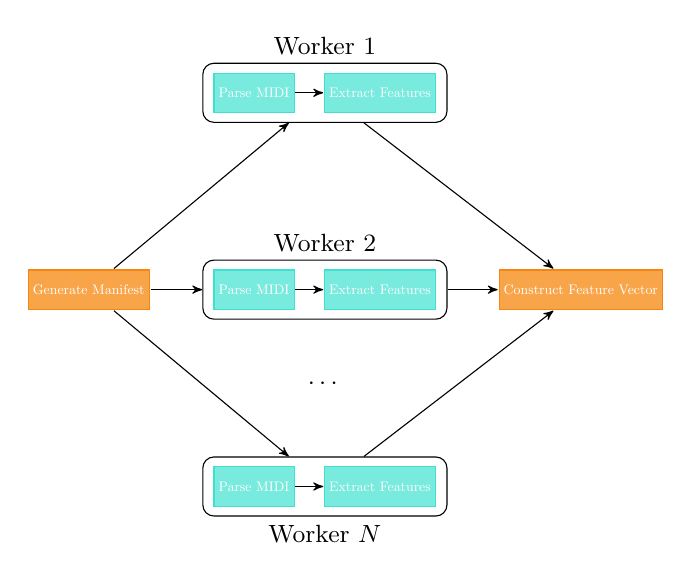
\begin{tikzpicture}[node distance=2cm,>=stealth']

      \tikzset{txtstyle/.style={text=black, font=\small}}
      \tikzstyle{workerbox} = [minimum width=3.1cm, minimum height=0.75cm, draw, thin, rounded corners, rectangle]

      \node[vertex style=BurntOrange,rectangle] (Source) {Generate Manifest};

      \begin{pgfonlayer}{background}
          \node[workerbox, right of=Source, above of=Source, xshift=1cm, yshift=0.5cm] (WB1) {};
          \node[workerbox, right of=Source, xshift=1cm] (WB2) {};
          \node[workerbox, below of=WB2, yshift=-0.5cm] (WBN) {};
      \end{pgfonlayer}

      \begin{scope}
          \node[txtstyle, above of=WB1, yshift=-1.4cm] (W1Label) {Worker 1};
          \node[vertex style=Turquoise,rectangle,below of=WB1, yshift=2cm, xshift=-1.8cm] (W11) {Parse MIDI};
          \node[vertex style=Turquoise,rectangle,right of=W11, xshift=1.2cm] (W12) {Extract Features};
      \end{scope}

      \begin{scope}
          \node[txtstyle, above of=WB2, yshift=-1.4cm] (W2Label) {Worker 2};
          \node[vertex style=Turquoise,rectangle,below of=WB2, yshift=2cm, xshift=-1.8cm] (W21) {Parse MIDI};
          \node[vertex style=Turquoise,rectangle,right of=W21, xshift=1.2cm] (W22) {Extract Features};
      \end{scope}

      \begin{scope}
          \node[txtstyle, above of=WBN, yshift=-2.6cm] (WNLabel) {Worker $N$};
          \node[txtstyle, above of=WNLabel, yshift=-0.1cm] (WNDots) {$\cdots$};
          \node[vertex style=Turquoise,rectangle,below of=WBN, yshift=2cm, xshift=-1.8cm] (WN1) {Parse MIDI};
          \node[vertex style=Turquoise,rectangle,right of=WN1, xshift=1.2cm] (WN2) {Extract Features};
      \end{scope}

      \node[vertex style=BurntOrange,rectangle,right of=WB2,xshift=4.5cm] (Sink) {Construct Feature Vector};

      \path[every node/.style={font=\sffamily\small}]
          (Source) edge[->] node {} (WB1)
          (Source) edge[->] node {} (WB2)
          (Source) edge[->] node {} (WBN)
          (W11) edge[->] node {} (W12)
          (W21) edge[->] node {} (W22)
          (WN1) edge[->] node {} (WN2)
          (WB1) edge[->] node {} (Sink)
          (WB2) edge[->] node {} (Sink)
          (WBN) edge[->] node {} (Sink);
          %(S) edge[->] node {} (Wn1);

      \end{tikzpicture}
      \caption{IPython Cluster}\label{fig:cluster}
\end{figure}

\subsection{Feature Extraction}

The features we have identified are
\begin{enumerate}
    \item 4-Tuples of successive notes
    \item 4-Tuples of successive durations
    \item 4-Tuples of successive normalized chords
\end{enumerate}

The feature vector is constructed by counting the number of occurrences of each tuple and normalizing.
The components of the vector are these normalized counts.

The extraction itself is performed in a distributed manner using the distributed computing capabilities of the IPython system~\cite{PERGRA}.
For every processor core we created a ``worker process''.
From the ``main process'' we send the file path to each MIDI file to a worker.
The worker then opens the file using the music21 library and extracts the necessary features.
Each worker then sends the extracted features back to the main process where the features are assembled into the feature vector.
The general topology and data flow of these processes are captured in Figure~\ref{fig:cluster}. 

\subsubsection{Note Vectors}\label{sec:vectors}
The first step in the construction is to extract a sequence of notes from a MIDI file.
Using the key signature of the piece and the circle of fifths (see Figure~\ref{fig:circleoffifths}) the notes are
mapped to numbers in the range $0-11$.
The result of this process is a sequence $S$ such that $S_i \in [12]$ (Where $[n]$ is the set of the first $n$ natural numbers.)

The second step is to construct $n$-tuples of consecutive notes.
Since there are only $12$ possible values a note may take,
there are $12^n$ possible tuples of length $n$.
Let $T$ denote these $12^n$ possible tuples,
where $T_0 = (0, \dots, 0), T_1 = (0, \dots, 1)$ and so on.
Let $S^n$ denote the sequence of $n$ consecutive notes taken over $S$.
That is,
\begin{equation*}
    S^n_i = t \iff S_i = t_0, \dots, S_{i + n - 1} = t_{n-1}
\end{equation*}
with $S_i = 0$ as appropriate when $\len{S} - n < i$.

In the final step, we construct the vector $\vec{x}$ of length $12^n$ where the $i$-th component of $\vec{x}$ is equal to the number of occurrences of the tuple $T_i$ in $S^n$.
That is,
\begin{equation*}
    \vec{x_i} = \len{\{ j : S_j^n = T_i \mathrm{\ for\ } 0 \leq j < \len{S^n} \}}
\end{equation*}

\subsubsection{Duration Vectors}
The construction of duration vectors is essentially the same as the
construction of note vectors.
In short, we extract the sequence of chords from a piece,
and then take the duration of each chord, quantize it,
and construct $n$-tuples of sequential durations.

This process results in a vector of size $k^n$, where $k$ depends on the quantization.
In our final implementation we used $k = 10$,
where a duration $d$ is assigned category $c - 1$ if and only if $c$ is the smallest integer such that $d > 1 / c$, for $0 < c \leq 10$.
If there is no such $c$, then $d$ is assigned to category $9$.

\subsubsection{Normal Chords\protect\footnote{We are indebted to Professor Haralick of the CUNY Graduate Center for suggesting this feature to us.}}\label{sec:chordgraph}
We define 192 \textit{normal chords}.
Figure~\ref{tab:chords} lists the sixteen normal chords with a tonic of $C$.
The remaining chords can be derived from the table by a relabeling of the circle of fifths (see Figure~\ref{fig:circleoffifths}).
\begin{figure}[h!]
\small
\begin{tabular}{lll}
\toprule
Name & Notes & Notation \\
\midrule
Major                   & 0, 4, 7         & $C$             \\
Minor                   & 0, 3, 7         & $C^{min}$       \\
Suspended               & 0, 5, 7         & $C^{sus}$       \\
Augmented               & 0, 4, 8         & $C^{aug}$       \\
Diminished              & 0, 3, 6         & $C^{dim}$       \\
Major Sixth             & 0, 4, 7, 9      & $C^{6}$         \\
Minor Sixth             & 0, 3, 7, 9      & $C^{min 6}$     \\
Dominant Seventh        & 0, 4, 7, 10     & $C^{7}$         \\
Major Seventh           & 0, 4, 7, 11     & $C^{M7}$        \\
Minor Seventh           & 0, 3, 7, 10     & $C^{min 7}$     \\
Half Diminished Seventh & 0, 3, 6, 10     & $C^{\phi 7}$    \\
Diminished Seventh      & 0, 3, 6, 9      & $C^{7}$         \\
Major Ninth             & 0, 4, 7, 11, 14 & $C^{M9}$        \\
Dominant Ninth          & 0, 4, 7, 10, 14 & $C^{9}$         \\
Dominant Minor Ninth    & 0, 4, 7, 10, 13 & $C^{7 \flat 9}$ \\
Minor Ninth             & 0, 3, 7, 10, 14 & $C^{min 9}$     \\
\bottomrule
\end{tabular}
\caption{Normal Chords}\label{tab:chords}
\end{figure}

Using unnormalized chords in the feature vector would not be tractable,
and so the motivation for normalization is ultimately pragmatic.
However, the normalization may be justifiable music theoretical grounds,
although a precise statement of the reasoning would take us too far afield.

We define a \textit{normalized chord} in the following way.
At each time slice\footnote{The granularity of the discretization is given by the time-signature of a piece.},
the notes which are currently being played constitute a chord.
Given a chord $c$ in key $k$ we then find the edit distance between $c$ and the normal chords with tonic $k$.
The named chord with tonic $k$ closest to $c$ (with ties broken lexically) is said to be the normalization of $c$.

The distance is computed with the Levenshtein distance using the circle of fifths and arithmetic modulo twelve.
Replacing a note in a chord with a note one half-step away has a cost of $w_1$ and removing a note from a chord has a cost of $w_2$.
For example, the distance between the note $C$ and $D^{\#}$ is $3w_1$,
as can readily be seen by consulting Figure~\ref{fig:circleoffifths}.
The distance between the chord $(0, 1)$ and $(0, 2, 1)$ is $w_2$, as the $2$ can be removed,
and removing either the $0$ or the $1$ results in a distance of at least $w_1 + w_2$.

A naive implementation would compute the distance between the chord being normalized and each of the normal chords.
If the size of the chord being normalized is $n$ and $m$ is the size of a normal chord then this operation is $O(nm)$.
Since the chords are all roughly the same size, this is essentially $O(n^2)$.
However, upper and lower bounds for the Levenshtein distance are trivial to compute,
and using these bounds we can limit the number of candidate chords during the normalization process.
For example, if $a, b$ and $c$ are chords, and the upper-bound for the distance between $a$ and $b$ is less than the lower-bound for the distance between $a$ and $c$, then there is no need to compute the actual distance between $a$ and $c$.
After this optimization the algorithm remains $O(n^2)$, but the constant is reduced significantly.

Once the chords have been normalized, we construct tuples in a manner similar to
the construction of the duration and note vectors, as documented in Section~\ref{sec:vectors}.

\begin{figure}[h!]
    \centering
    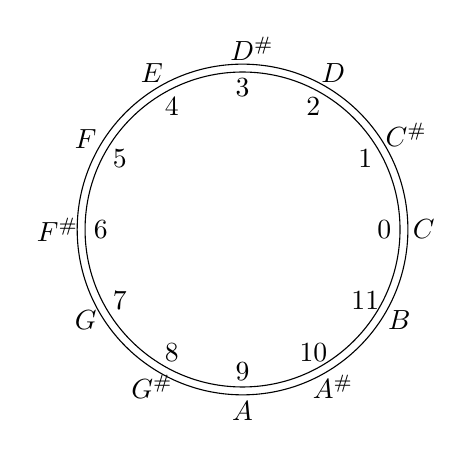
\begin{tikzpicture}
        \draw (0,0) circle (2cm);
        \draw (0,0) circle (2.1cm);
        \node at (0:2.3) {$C$};
        \node at (0:1.8) {$0$};

        \node at (30:2.4) {$C^{\#}$};
        \node at (30:1.8) {$1$};

        \node at (60:2.3) {$D$};
        \node at (60:1.8) {$2$};

        \node at (87:2.3) {$D^{\#}$};
        \node at (90:1.8) {$3$};

        \node at (120:2.3) {$E$};
        \node at (120:1.8) {$4$};

        \node at (150:2.3) {$F$};
        \node at (150:1.8) {$5$};

        \node at (180:2.35) {$F^{\#}$};
        \node at (180:1.8) {$6$};

        \node at (210:2.3) {$G$};
        \node at (210:1.8) {$7$};

        \node at (240:2.3) {$G^{\#}$};
        \node at (240:1.8) {$8$};

        \node at (270:2.3) {$A$};
        \node at (270:1.8) {$9$};

        \node at (300:2.3) {$A^{\#}$};
        \node at (300:1.8) {$10$};

        \node at (330:2.3) {$B$};
        \node at (330:1.8) {$11$};
    \end{tikzpicture}
    \caption{Circle of Fifths}\label{fig:circleoffifths}
\end{figure}

\section{Methods}

Due to the significant sizes of the vectors, $14^4$, $12^4$ and $10^4$,
we decided to use the simplest classifiers which we believed to be capable of
the required accuracy.

\subsection{Support Vector Machine}
A \textit{Support Vector Machine} (SVM),
introduced in~\cite{vapnik1963pattern},
is an algorithm that given a data set in a high dimensional space,
constructs a hyperplane that separates the data points in that set into two classes.
We refer to the original SVM algorithm as a \textit{Hard Margin Support Vector Machine} (HMSVM).
The hyperplane constructed by a HMSVM must classify all data points correctly;
i.e.\ there can be no data points that wind up being classified incorrectly.

\subsection{Soft Margin Support Vector Machine}
A \textit{Soft Margin Support Vector Machine} (SMSVM),
introduced in~\cite{Cortes1995},
is a Support Vector Machine in which the hyperplane used to separate the data points into classes may place a few points into incorrect classes.
A SMSVM is particularly useful in data sets with high levels of noise,
because an SMSVM is better at ignoring outliers and avoiding skewing of classification because of outliers.

In symbols, the objective of a SSVM is to solve
\begin{equation*}
    \min_{\beta_0, \beta} \Big\{ \frac{1}{n} \sum_{i=1}{n} \max (0, 1 - y_i (\vec{w} \dot \vec{x_i} - b)) \Big\} + \lambda \Bigg(\sum_{j=1}^p \len{\vec{w}}\Bigg)^2
\end{equation*}
where $\gamma$ can be thought of as representing the relationship between margin size and the correctness of the classification
(Low values of $\gamma$ are equivalent to HMSVMs).

\subsection{LASSO}
The \textit{Least Absolute Selection and Shrinkage Operator} (LASSO),
introduced in~\cite{tibshirani1996regression},
is an algorithm that takes a linear regression of the data,
and uses it to enforces a constraint of the model's parameters,
while setting a specific constant as the upper bound on the sum of absolute values.
The LASSO algorithm shrinks the model so that variables that minimize prediction error are identified.
Because of this, LASSO is also called a \textit{Shrinkage and Variable Selection Method}.

In symbols, the objective of the LASSO is to solve
\begin{equation*}
    \min_{\beta_0, \beta} \Big\{ \frac{1}{n} \sum_{i=1}{n} {(y_i - \beta_0 x_i^t \beta)}^2 \Big\} \mathrm{\ subject\ to\ } \sum_{j=1}^p \len{\beta_j} \leq t
\end{equation*}
where the parameter $t$ gives the amount of regularisation.

\section{Results}

We used 144 MIDI files in total: 72 files from the 1970s and 72 files from the 1980s.
Due to the limitations of the music21 library it was computationally expensive to process more files.
In all of our experiments we used the following break down of the vectors into Training, Test, and Validation sets.

\begin{figure}[h!]
\centering
\begin{tabular}{lrr}
\toprule
Set        & Percent of Total & Number of Files \\
\midrule
Test       &             15\% &              25 \\
Training   &             85\% &              97 \\
Validation &             10\% &              22 \\
\midrule
\textbf{Total} &        100\% &             144 \\
\bottomrule
\end{tabular}
\end{figure}

Following the practical guide~\cite{hsu2003practical} for selecting SVM parameters for $c$ and $\gamma$
(though we were only fitting the $c$ and the polynomial degree), we used $c$ in range $e^k$,
for $k \in [-10, 2*degee]$.

\subsection{Soft Margin SVM}
\subsubsection{Normalized Chords}
In our first experiment we tested with 4-tuples of normalized chords.
\begin{figure}[h!]
\centering
\begin{tabular}{lr}
\toprule
Set        & Accuracy \\
\midrule
Test       &     95\% \\
Training   &     98\% \\
Validation &     92\% \\
\bottomrule
\end{tabular}
\end{figure}

The found parameter $c$ is equal to $283.79$,
the degree of the best polynomial fit is 4.
Figure~\ref{fig:exp1} gives the plots for the variation of the parameter $c$ versus the validation set accuracy for each degree of the polynomial,
along with the resulting confusion matrices.

\subsubsection{Pitchs}
In our second experiment we used $4$-tuples of pitchs.
\begin{figure}[h!]
\centering
\begin{tabular}{lr}
\toprule
Set        & Accuracy \\
\midrule
Test       &    100\% \\
Training   &    100\% \\
Validation &     96\% \\
\bottomrule
\end{tabular}
\end{figure}

The found parameter $c$ is equal to $2980.96$,
the degree of the best polynomial fit is 4. Figure~\ref{fig:exp2} shows the
plots for the change of the accuracy of the fit based on the parameter $c$,
along with the corresponding confusion matrices.

\subsubsection{Durations}
In our third experiment we used $4$-tuples of durations.
\begin{figure}[h!]
\centering
\begin{tabular}{lr}
\toprule
Set        & Accuracy \\
\midrule
Test       &    50\% \\
Training   &    61\% \\
Validation &    50\% \\
\bottomrule
\end{tabular}
\end{figure}

As one might expect, the durations alone are essentialy random.

The found parameter $c$ is equal to $0$,
and the degree of the best polynomial fit is 1.
Figure~\ref{fig:exp3} shows the plots for the change of the accuracy of the fit based on the parameter $c$, along with the corresponding confusion matrices.

\subsection{LASSO}
\subsubsection{Normalized Chords}
In our third experiment we again use $4$-tuples of normalized chords.
\begin{figure}[h!]
\centering
\begin{tabular}{lr}
\toprule
Set        & Accuracy \\
\midrule
Test       &     86\% \\
Training   &     98\% \\
Validation &     92\% \\
\bottomrule
\end{tabular}
\end{figure}

The found parameter $\alpha$ is equal to $0.04$.
Figure~\ref{fig:exp4} demonstrates the plots for the dependency of the accuracy of the model on the parameter for the validation set,
along with the resulting confusion matrices.

\subsubsection{Pitches}
In our fifth experiment we use $4$-tuples of pitches.
\begin{figure}[H]
\centering
\begin{tabular}{lr}
\toprule
Set        & Accuracy  \\
\midrule
Test       &     86\%  \\
Training   &     100\% \\
Validation &     96\%  \\
\bottomrule
\end{tabular}
\end{figure}

The found parameter $\alpha$ is equal to $0$.
Figure~\ref{fig:exp5} shows the plot for the dependency of the accuracy of the model on the parameter $\alpha$ for the validation set,
along with the resulting confusion matrices.

\subsubsection{Durations}
In our sixth and final experiment we use $4$-tuples of durations.
\begin{figure}[H]
\centering
\begin{tabular}{lr}
\toprule
Set        & Accuracy \\
\midrule
Test       &     50\% \\
Training   &     73\% \\
Validation &     50\% \\
\bottomrule
\end{tabular}
\end{figure}

The found parameter $\alpha$ is equal to $0$.
The LASSO method does not fare any better against (essentially) random data than does the SSVM method.
Figure~\ref{fig:exp6} shows the plot for the dependency of the accuracy of the model on the parameter $\alpha$ for the validation set,
along with the resulting confusion matrices.

\section{Conclusion}

In this paper we compare two methods for performing a binary classification of
the genre of US pop songs from the 1970's and 1980's.
We identify two features,
pitches and normalized chords,
which we use to classify songs with accuracies of 98\% and 100\%, respectivly.
We also identify a feature, chord duration, which while interesting from a
musical perspective, fails to aid these methods in the classification of songs.
We summarize our results in Figure~\ref{tbl:summary}
\begin{figure}[H]
\centering
\begin{tabular}{lccc}
\toprule
    \multirow{2}[2]{*}{\hspace{5mm} Set} & \multicolumn{3}{c}{SSVM} \\
\cmidrule(lr){2-4}
    & Chords & Pitches & Durations \\
\midrule
    Test       &     95\% & 100\% & 50\% \\
    Training   &     98\% & 100\% & 61\% \\
    Validation &     92\% & 96\%  & 50\% \\
\bottomrule
\end{tabular}
\end{figure}

\begin{figure}[H]
\centering
\begin{tabular}{lccc}
\toprule
    \multirow{2}[2]{*}{\hspace{5mm} Set} & \multicolumn{3}{c}{LASSO} \\
\cmidrule(lr){2-4}
    & Chords & Pitches & Durations \\
\midrule
    Test       &     86\% & 86\%  & 50\% \\
    Training   &     98\% & 100\% & 73\% \\
    Validation &     92\% & 96\%  & 50\% \\
\bottomrule
\end{tabular}
\caption{Results Summary}\label{tbl:summary}
\end{figure}

It would be interesting to extend this work to use additional features,
and to perform a more general $k$-ary classification.
It would also be somewhat interesting to see the results of unsupervised
learning on these features, although this would obviously have fewer real
world applications.

All of our generated data and code is available for viewing and download~\cite{Cuspian}.

\begin{figure}
    \centering
    \includegraphics[scale=0.41]{SVMChords.png}
    \includegraphics[scale=0.4]{SVMChordsConfusion.png}
    \includegraphics[scale=0.4]{SVMChordsConfusionNorm.png}
    \caption{First Experiment}\label{fig:exp1}
\end{figure}

\begin{figure}
    \centering
    \includegraphics[scale=0.41]{SVMPitches.png}
    \includegraphics[scale=0.4]{SVMPitchesConfusion.png}
    \includegraphics[scale=0.4]{SVMPitchesConfusionNorm.png}
    \caption{Second Experiment}\label{fig:exp2}
\end{figure}

\begin{figure}
    \centering
    \includegraphics[scale=0.41]{SVMDurations.png}
    \includegraphics[scale=0.4]{SVMDurationsConfusion.png}
    \includegraphics[scale=0.4]{SVMDurationsConfusionNorm.png}
    \caption{Third Experiment}\label{fig:exp3}
\end{figure}

\begin{figure}
    \centering
    \includegraphics[scale=0.41]{LASSOChords.png}
    \includegraphics[scale=0.4]{LASSOChordsConfusion.png}
    \includegraphics[scale=0.4]{LASSOChordsConfusionNorm.png}
    \caption{Fourth Experiment}\label{fig:exp4}
\end{figure}

\begin{figure}
    \centering
    \includegraphics[scale=0.41]{LASSOPitches.png}
    \includegraphics[scale=0.4]{LASSOPitchesConfusion.png}
    \includegraphics[scale=0.4]{LASSOPitchesConfusionNorm.png}
    \caption{Fifth Experiment}\label{fig:exp5}
\end{figure}

\begin{figure}
    \centering
    \includegraphics[scale=0.41]{LASSODurations.png}
    \includegraphics[scale=0.4]{LASSODurationsConfusion.png}
    \includegraphics[scale=0.4]{LASSODurationsConfusionNorm.png}
    \caption{Sixth Experiment}\label{fig:exp6}
\end{figure}

\printbibliography[]

\end{document}

